\documentclass[journal,12pt,twocolumn]{IEEEtran}
\usepackage{setspace}
\usepackage{gensymb}
\singlespacing
\usepackage[cmex10]{amsmath}
\usepackage{amsthm}
\usepackage{mathrsfs}
\usepackage{txfonts}
\usepackage{stfloats}
\usepackage{bm}
\usepackage{cite}
\usepackage{cases}
\usepackage{subfig}
\usepackage{longtable}
\usepackage{multirow}
\usepackage{enumitem}
\usepackage{mathtools}
\usepackage{steinmetz}
\usepackage{tikz}
\usepackage{circuitikz}
\usepackage{verbatim}
\usepackage{tfrupee}
\usepackage[breaklinks=true]{hyperref}
\usepackage{tkz-euclide}
\usetikzlibrary{calc,math}
\usepackage{listings}
    \usepackage{color}                                            %%
    \usepackage{array}                                            %%
    \usepackage{longtable}                                        %%
    \usepackage{calc}                                             %%
    \usepackage{multirow}                                         %%
    \usepackage{hhline}                                           %%
    \usepackage{ifthen}                                           %%
  %optionally (for landscape tables embedded in another document): %%
    \usepackage{lscape}     
\usepackage{multicol}
\usepackage{chngcntr}
\DeclareMathOperator*{\Res}{Res}
\renewcommand\thesection{\arabic{section}}
\renewcommand\thesubsection{\thesection.\arabic{subsection}}
\renewcommand\thesubsubsection{\thesubsection.\arabic{subsubsection}}

\renewcommand\thesectiondis{\arabic{section}}
\renewcommand\thesubsectiondis{\thesectiondis.\arabic{subsection}}
\renewcommand\thesubsubsectiondis{\thesubsectiondis.\arabic{subsubsection}}

% correct bad hyphenation here
\hyphenation{op-tical net-works semi-conduc-tor}
\def\inputGnumericTable{}                                 %%

\lstset{
frame=single, 
breaklines=true,
columns=fullflexible
}

\begin{document}


\newtheorem{theorem}{Theorem}[section]
\newtheorem{problem}{Problem}
\newtheorem{proposition}{Proposition}[section]
\newtheorem{lemma}{Lemma}[section]
\newtheorem{corollary}[theorem]{Corollary}
\newtheorem{example}{Example}[section]
\newtheorem{definition}[problem]{Definition}
\newcommand{\BEQA}{\begin{eqnarray}}
\newcommand{\EEQA}{\end{eqnarray}}
\newcommand{\define}{\stackrel{\triangle}{=}}

\bibliographystyle{IEEEtran}
\providecommand{\mbf}{\mathbf}
\providecommand{\pr}[1]{\ensuremath{\Pr\left(#1\right)}}
\providecommand{\qfunc}[1]{\ensuremath{Q\left(#1\right)}}
\providecommand{\sbrak}[1]{\ensuremath{{}\left[#1\right]}}
\providecommand{\lsbrak}[1]{\ensuremath{{}\left[#1\right.}}
\providecommand{\rsbrak}[1]{\ensuremath{{}\left.#1\right]}}
\providecommand{\brak}[1]{\ensuremath{\left(#1\right)}}
\providecommand{\lbrak}[1]{\ensuremath{\left(#1\right.}}
\providecommand{\rbrak}[1]{\ensuremath{\left.#1\right)}}
\providecommand{\cbrak}[1]{\ensuremath{\left\{#1\right\}}}
\providecommand{\lcbrak}[1]{\ensuremath{\left\{#1\right.}}
\providecommand{\rcbrak}[1]{\ensuremath{\left.#1\right\}}}
\theoremstyle{remark}
\newtheorem{rem}{Remark}
\newcommand{\sgn}{\mathop{\mathrm{sgn}}}
\providecommand{\abs}[1]{\left\vert#1\right\vert}
\providecommand{\res}[1]{\Res\displaylimits_{#1}} 
\providecommand{\norm}[1]{\left\lVert#1\right\rVert}
\providecommand{\mtx}[1]{\mathbf{#1}}
\providecommand{\mean}[1]{E\left[ #1 \right]}
\providecommand{\fourier}{\overset{\mathcal{F}}{ \rightleftharpoons}}
\providecommand{\system}{\overset{\mathcal{H}}{ \longleftrightarrow}}
\newcommand{\solution}{\noindent \textbf{Solution: }}
\newcommand{\cosec}{\,\text{cosec}\,}
\providecommand{\dec}[2]{\ensuremath{\overset{#1}{\underset{#2}{\gtrless}}}}
\newcommand{\myvec}[1]{\ensuremath{\begin{pmatrix}#1\end{pmatrix}}}
\newcommand{\mydet}[1]{\ensuremath{\begin{vmatrix}#1\end{vmatrix}}}
\numberwithin{equation}{subsection}
\makeatletter
\@addtoreset{figure}{problem}
\makeatother

\let\StandardTheFigure\thefigure
\let\vec\mathbf
\renewcommand{\thefigure}{\theproblem}



\def\putbox#1#2#3{\makebox[0in][l]{\makebox[#1][l]{}\raisebox{\baselineskip}[0in][0in]{\raisebox{#2}[0in][0in]{#3}}}}
     \def\rightbox#1{\makebox[0in][r]{#1}}
     \def\centbox#1{\makebox[0in]{#1}}
     \def\topbox#1{\raisebox{-\baselineskip}[0in][0in]{#1}}
     \def\midbox#1{\raisebox{-0.5\baselineskip}[0in][0in]{#1}}

\vspace{3cm}


\title{Assignment 1}
\author{Jaswanth Chowdary Madala}





% make the title area
\maketitle

\newpage

%\tableofcontents

\bigskip

\renewcommand{\thefigure}{\theenumi}
\renewcommand{\thetable}{\theenumi}


\begin{enumerate}
\item Find the equation of the ellipse that satisfies the conditions - Centre at $\brak{0,0}$, major axis on the y-axis and passes through the points $\brak{3,2}$ and $\brak{1,6}$.
%\begin{figure}[ht]
%\centering
%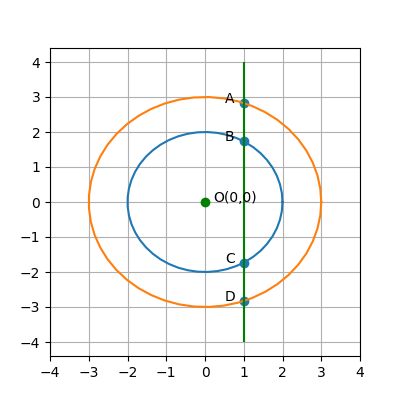
\includegraphics[width = \columnwidth]{"./figs/fig.png"}
%\caption{Graph}
%\label{fig:1}
%\end{figure}

\textbf{Solution:}
The equation of the conic with focus $\vec{F}$, directrix $\vec{n}^\top\vec{x} = c$ and eccentricity $e$ is given by
\begin{align}
\vec{x}^\top\vec{V}\vec{x} + 2\vec{u}^\top\vec{x} + f = 0
\label{eq:1}
\end{align}
where
\begin{align}
\vec{V} &\triangleq \norm{\vec{n}}^2\vec{I} - e^2\vec{n}\vec{n}^\top \label{eq:2} \\
\vec{u} &\triangleq ce^2\vec{n} - \norm{\vec{n}}^2\vec{F} \label{eq:3} \\
f &\triangleq \norm{\vec{n}}^2\norm{\vec{F}}^2 - c^2e^2 \label{eq:4}
\end{align}
Given that the conic is an ellipse with major axis along the $y$-axis, we get
\begin{align}
\vec{n} = \myvec{0\\1}
\end{align}
Thus,
\begin{align}
\vec{V} = \myvec{1&0\\0&1-e^2} \label{eq:5} \\
\vec{u} = ce^2\myvec{0\\1} - \vec{F} \label{eq:6} \\
f = \norm{\vec{F}}^2 - c^2e^2 \label{eq:7}
\end{align}
The centre of the conic is given by
\begin{align}
\vec{c} = -\vec{V}^{-1}\vec{u}
\label{eq:8}
\end{align}
Since $\vec{c} = \vec{0}$ and $\vec{V}^{-1} \neq \vec{0}$, it follows from \eqref{eq:8} that 
\begin{align}
\vec{u} = \vec{0}
\end{align}
Thus, from \eqref{eq:6},
\begin{align}
\vec{F} = \myvec{0\\ce^2}
\label{eq:9}
\end{align}
and so,
\begin{align}
f = c^2e^2\brak{e^2-1}
\label{eq:9}
\end{align}
Given that the conic passes throught point,
\begin{align}
\vec{P} = \myvec{3\\2} 
\end{align}
Putting $\vec{x} = \vec{P}$ in \eqref{eq:1} we get,
\begin{align}
\myvec{3&2}\myvec{1&0\\0&1-e^2}\myvec{3\\2} + f &= 0 \\
\implies 4e^2 - f = 13 \label{eq:10}
\end{align}
Given that the conic passes throught point,
\begin{align}
\vec{Q} = \myvec{1\\6} 
\end{align}
Putting $\vec{x} = \vec{Q}$ in \eqref{eq:1}, we get
\begin{align}
\myvec{1&6}\myvec{1&0\\0&1-e^2}\myvec{1\\6} + f &= 0 \\
\implies 36e^2 - f = 37 \label{eq:11}
\end{align}
The equations \eqref{eq:10} and \eqref{eq:11} can be formulated as the following matrix equation
\begin{align}
\myvec{4&-1\\36&-1}\myvec{e^2\\f} = \myvec{13\\37}
\label{eq:12}
\end{align}
The augmented matrix is given by,
\begin{align}
\myvec{4&-1&\vline&13\\36&-1&\vline&37}
\end{align}
\begin{align}
\xleftrightarrow[]{R_1\leftarrow R_1-R_2} &\myvec{-32&0&\vline&-24\\36&-1&\vline&37} \\
\xleftrightarrow[]{R_1\leftarrow-\frac{R_1}{8}}& \myvec{4&0&\vline&3\\36&-1&\vline&37} \\
\xleftrightarrow[]{R_2\leftarrow R_2-9R_1}
&\myvec{4&0&\vline&3\\0&-1&\vline&10} \\
\xleftrightarrow[R_2\leftarrow -R_2]{R_1\leftarrow \frac{R_1}{4}}
&\myvec{1&0&\vline&\frac{3}{4}\\0&1&\vline&-10}
\end{align}
Thus,
\begin{align}
e^2 = \frac{3}{4},\ f = -10
\end{align}
The equation of the conic is given by
\begin{align}
\vec{x}^\top\myvec{1&0\\0&\frac{1}{4}}\vec{x} - 10 = 0
\end{align}
\begin{figure}[ht]
\centering
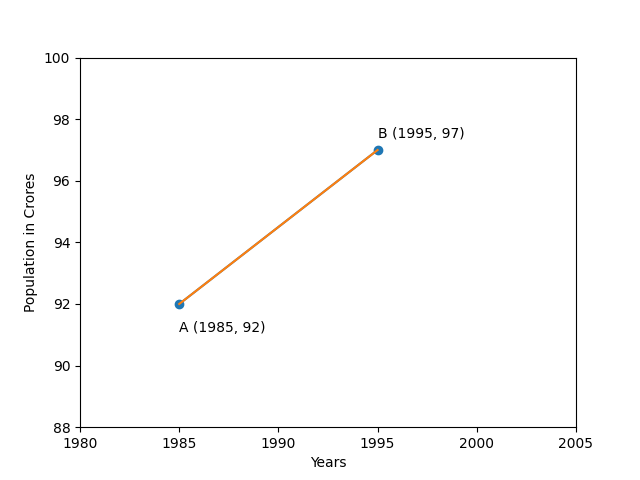
\includegraphics[width = \columnwidth]{"./figs/fig1.png"}
\caption{Graph}
\label{fig:1}
\end{figure}
\begin{table}[h]
\centering
%%%%%%%%%%%%%%%%%%%%%%%%%%%%%%%%%%%%%%%%%%%%%%%%%%%%%%%%%%%%%%%%%%%%%%
%%                                                                  %%
%%  This is a LaTeX2e table fragment exported from Gnumeric.        %%
%%                                                                  %%
%%%%%%%%%%%%%%%%%%%%%%%%%%%%%%%%%%%%%%%%%%%%%%%%%%%%%%%%%%%%%%%%%%%%%%

\begin{center}
\begin{tabular}{|c|c|c|}
\hline
\textbf{RV}& \textbf{Values} & \textbf{Description} \\ \hline
$X$		   & 	$\{0,1\}$	&  1st draw - 0: black card, 1: red card\\ \hline
$Y$ 		   & 	$\{0,1\}$	&  2nd draw - 0: black card, 1: red card\\ \hline
$X,Y$ 		   & 	$\{00\}$	&	2 cards drawn are black\\ \hline
\end{tabular}
\end{center}

\caption{}
\label{tab:1}
\end{table}
\end{enumerate}
\end{document}